% Quick settings:
% - use `onehalf` for 1.5 line spacing or `double` for 2.0;
% - use `redaccent` (default) or `blackaccent` for black hyperlinks.
\documentclass[onehalf,redaccent]{polyu-thesis}

% Thesis metadata and optional sections.
% Edit thesis metadata and optional sections here.

\newcommand{\thesistitle}{Thesis Title}
\newcommand{\studentname}{Full Name of Student}
\newcommand{\degree}{Doctor of Philosophy}
\newcommand{\degreeabbr}{PhD}
\newcommand{\department}{Name of Department}

% Use the initial submission month and year, even in the final thesis.
\newcommand{\initialsubmissionmonth}{Month}
\newcommand{\initialsubmissionyear}{20XX}
\newcommand{\awardyear}{20XX}

\newcommand{\chiefsupervisor}{Name of Chief Supervisor}

% Replace this space with an electronic signature if needed:
% \renewcommand{\studentsignature}{\includegraphics[height=15mm]{signature.pdf}}
\newcommand{\studentsignature}{\rule{0pt}{16mm}}

% Use true for examination and false for the final corrected thesis.
\newif\ifinitialsubmission
\initialsubmissiontrue

% For a dual PhD, set true and complete both fields.
\newif\ifdualdegree
\dualdegreefalse
\newcommand{\partneruniversity}{Name of Partner University}
\newcommand{\partnerdepartment}{Name of Department at Partner University}

% Transfer-in PhD students must enable the attribution statement.
\newif\iftransferin
\transferinfalse
\newcommand{\polyuworkchapters}{X--Y}
\newcommand{\previousuniversity}{Name of Previous University}

% Set a flag to false to omit that section.
\newif\ifdedication
\dedicationtrue % Use \dedicationfalse to omit the dedication.
\newif\ifpublications
\publicationstrue % Use \publicationsfalse to omit the publications page.
\newif\iflistoffigures
\listoffigurestrue % Use \listoffiguresfalse to omit the List of Figures.
\newif\iflistoftables
\listoftablestrue % Use \listoftablesfalse to omit the List of Tables.
\newif\iflistofalgorithms
\listofalgorithmstrue % Use \listofalgorithmsfalse to omit the algorithm list.
\newif\iflistoflistings
\listoflistingstrue % Use \listoflistingsfalse to omit the code-listing list.
\newif\ifabbreviations
\abbreviationstrue % Use \abbreviationsfalse to omit abbreviations.

% User packages, bibliography, and PDF metadata.
% Add user packages, bibliography settings, and PDF metadata here.

\usepackage[
  backend=biber,
  style=numeric-comp,
  sorting=nyt,
  sortcites=true,
  giveninits=true,
  uniquename=init,
  maxbibnames=99
]{biblatex}
\addbibresource{references.bib}

\hypersetup{
  pdftitle={\thesistitle},
  pdfauthor={\studentname},
  pdfsubject={Thesis submitted for the degree of \degree},
  pdfcreator={LaTeX with the PolyU Thesis LaTeX template}
}


\begin{document}

% Required opening pages.
\pagenumbering{gobble}
\hypersetup{pageanchor=false}
\makecoverpage
\makethesistitlepage
% Keep the declaration text consistent with the current PolyU RPg Handbook.
\thispagestyle{empty}
\begin{center}
  \vspace*{12mm}
  {\Large\rmfamily\bfseries CERTIFICATE OF ORIGINALITY\par}
\end{center}

\vspace{18mm}

I hereby declare that this thesis is my own work and that, to the best of my knowledge and belief, it reproduces no material previously published or written, nor material that has been accepted for the award of any other degree or diploma, except where due acknowledgement has been made in the text.

\vspace{24mm}

\noindent
\begin{minipage}[t]{0.42\textwidth}
  \centering
  \studentsignature\par
  \vspace{1mm}\hrule
  \vspace{1mm}(Signed)
\end{minipage}
\hfill
\begin{minipage}[t]{0.42\textwidth}
  \centering
  \rule{0pt}{16mm}\studentname\par
  \vspace{1mm}\hrule
  \vspace{1mm}(Name of student)
\end{minipage}

\clearpage

\iftransferin
  % Required only for transfer-in PhD students; enable it in metadata.tex.
\thispagestyle{empty}
\begin{center}
  \vspace*{8mm}
  {\Large\rmfamily\bfseries STATEMENT OF RESEARCH ATTRIBUTION AND INTELLECTUAL PROPERTY CLEARANCE\par}
\end{center}

\vspace{14mm}

This thesis incorporates research conducted both prior to and during my registration as a PhD student at The Hong Kong Polytechnic University (PolyU). I hereby confirm that Chapters \polyuworkchapters\ of this thesis were completed at PolyU under the supervision of \chiefsupervisor.

\vspace{1em}

All other content of this thesis was completed at \previousuniversity, and I have obtained full and proper clearance for all intellectual property (IP) and research data derived from or employed in the research conducted at \previousuniversity.

\vspace{24mm}

\noindent
\begin{minipage}[t]{0.42\textwidth}
  \centering
  \studentsignature\par
  \vspace{1mm}\hrule
  \vspace{1mm}(Signed)
\end{minipage}
\hfill
\begin{minipage}[t]{0.42\textwidth}
  \centering
  \rule{0pt}{16mm}\studentname\par
  \vspace{1mm}\hrule
  \vspace{1mm}(Name of student)
\end{minipage}

\clearpage

\fi

% Front matter uses lower-case Roman numerals.
\hypersetup{pageanchor=true}
\thesisfrontmatter
\ifdedication
  \thesisfrontchapter{Dedication}

% Keep the dedication concise, or disable it in metadata.tex.
To my family.

\fi
\thesisfrontchapter{Abstract}

% PolyU requires 200--500 words. Replace this example before submission.
This thesis investigates a clearly defined research problem whose practical importance and unresolved scientific questions motivate the work. It begins by reviewing the relevant theoretical foundations and empirical evidence, identifying limitations in existing approaches and establishing the research questions addressed in the subsequent chapters. A reproducible methodology is then developed to examine these questions using appropriate data, experimental controls, evaluation measures, and statistical analyses. The proposed approach is compared with established baselines under consistent conditions, while additional experiments examine robustness, sensitivity to design choices, and the influence of the principal assumptions. The results demonstrate how the selected methodology addresses the stated research objectives and clarify the circumstances in which its advantages and limitations become most apparent. The discussion relates the findings to prior research, considers alternative explanations, and distinguishes conclusions supported directly by evidence from interpretations that require further validation. Particular attention is given to reproducibility, uncertainty, generalisability, ethical considerations, and the practical implications of the work. Taken together, the studies provide a coherent contribution to the field and establish a foundation for subsequent investigation. Future research should extend the evaluation to additional settings, test the approach using independent evidence, and examine how the identified limitations can be mitigated. Replace this anonymous example with a self-contained summary of the completed thesis, including its actual problem, methods, principal quantitative findings, conclusions, and significance.

\ifpublications
  \thesisfrontchapter{Publications Arising from the Thesis}

% This page is optional. Enable it in metadata.tex after replacing this sample.
% PolyU asks for entries in alphabetical order of the first author.
\begin{enumerate}[leftmargin=*]
  \item Author, A. A., and Collaborator, B. B. (20XX). Title of the first publication arising from the thesis. \emph{Journal Name}, volume, pages.
  \item Author, A. A., Collaborator, B. B., and Researcher, C. C. (20XX). Title of the second publication arising from the thesis. \emph{Conference or Journal Name}, pages.
\end{enumerate}

\fi
\thesisfrontchapter{Acknowledgements}

I gratefully acknowledge \chiefsupervisor, my Chief Supervisor, for guidance, advice, and supervision throughout this research. I also acknowledge the collaborators and colleagues whose contributions are identified in the relevant chapters and cited where appropriate. Replace this text before submission so that every contribution by supervisors, former supervisors, advisers, collaborators, technical staff, and others is declared accurately.


\clearpage
\tableofcontents
\iflistoffigures
  \clearpage
  \listoffigures
\fi
\iflistoftables
  \clearpage
  \listoftables
\fi
\iflistofalgorithms
  \clearpage
  \listofalgorithms
\fi
\iflistoflistings
  \clearpage
  \lstlistoflistings
\fi
\ifabbreviations
  \thesisfrontchapter{List of Abbreviations}

\begin{longtable}{@{}p{0.20\textwidth}p{0.72\textwidth}@{}}
  \toprule
  \textbf{Abbreviation} & \textbf{Meaning} \\
  \midrule
  \endhead
  API  & Application programming interface \\
  DOI  & Digital object identifier \\
  PDF  & Portable Document Format \\
  RPg  & Research postgraduate \\
  \bottomrule
\end{longtable}


\fi

% Main matter uses Arabic page numbers.
\thesismainmatter
\chapter{Introduction}
\label{ch:introduction}

\section{Background}

The introduction should establish the problem, its significance, and the context
needed to understand the thesis. Begin with the broader research area, narrow the
discussion to the specific problem, and define the scope of the investigation.
Avoid turning this section into a second literature review; reserve detailed
comparison of prior methods for \Cref{ch:literature-review}.

Factual claims should be supported by appropriate sources. This sentence
demonstrates a compressed numeric citation \parencite{example2025,example2024};
citations appear as bracketed numbers such as [1] in the compiled thesis.

\section{Aim and Objectives}

State the overall aim in one precise sentence, then translate it into objectives
that can be evaluated by the methods and results. Each objective should correspond
to a later methodological step and a reported finding.

An objectives list can be used when it improves readability:

\begin{enumerate}[label=\textbf{O\arabic*:},leftmargin=*]
  \item define a reproducible problem setting;
  \item compare representative methods under consistent conditions; and
  \item analyse uncertainty, limitations, and generalisability.
\end{enumerate}

\subsection{Research Questions}

Research questions should be specific, answerable, and aligned with the objectives.
If hypotheses are used, state them after the relevant question and define the
evidence that would support or challenge each one.

\subsubsection{Scope and Terminology}

Define the population, data, task, and evaluation boundary that apply throughout
the thesis. Introduce specialised terms once and use them consistently; a glossary
or abbreviation list is preferable when many recurring terms are required.

Technical terms may be clarified in a footnote.\footnote{Footnotes should be concise and should not be used as a substitute for essential argumentation or citation.}

\section{Thesis Organisation}

\Cref{ch:literature-review} reviews the relevant literature. \Cref{ch:study-one}
demonstrates a self-contained study with its own introduction, methods, results,
and discussion. \Cref{ch:conclusions} integrates the conclusions and identifies
directions for future research.

\chapter{Literature Review}
\label{ch:literature-review}

\section{Conceptual Foundations}

This section should introduce the theories, definitions, and assumptions on which
the research depends. Organise the discussion by concepts or research questions
rather than presenting one summary paragraph per paper. Where definitions vary,
explain which interpretation the thesis adopts and why.

A strong review synthesises evidence across studies. It should identify areas of
agreement, explain conflicting findings, and distinguish limitations in available
data from limitations in methods or evaluation design.

\section{Representative Approaches}

Compare representative approaches using criteria that matter to the thesis, such
as data requirements, assumptions, reproducibility, external validation, and
computational cost. The comparison should make the rationale for the chosen
methodology transparent rather than merely declaring one family of methods to be
superior.

\begin{sidewaystable}[p]
  \centering
  \scriptsize
  \caption[Example wide literature comparison.]{Example wide literature comparison with placeholder data. A short, plain optional caption is supplied for the List of Tables, while this longer caption may contain the detail needed to interpret the table.}
  \label{tab:wide-review}
  \begin{tabularx}{0.92\textheight}{@{}L{31mm}*{7}{>{\centering\arraybackslash}X}@{}}
    \toprule
    \textbf{Study} & \textbf{Setting} & \textbf{Data} & \textbf{Design} & \textbf{Primary metric} & \textbf{External test} & \textbf{Code} & \textbf{Key limitation} \\
    \midrule
    Example A \parencite{example2024} & Laboratory & Public & Retrospective & Accuracy & No & Yes & Single-site evaluation \\
    Example B \parencite{example2025} & Simulation & Synthetic & Controlled & Error & Yes & No & Limited sensitivity analysis \\
    Example C & Field study & Mixed & Prospective & Utility & Partial & Yes & Small sample size \\
    Example D & Benchmark & Public & Cross-sectional & Score & No & Partial & Narrow task definition \\
    Proposed study & Multiple settings & Mixed & Reproducible & Several metrics & Yes & Yes & Replace with actual limitations \\
    \bottomrule
  \end{tabularx}
\end{sidewaystable}


\section{Research Gap}

Conclude the review by identifying a focused and defensible gap. State what remains
unknown, why existing evidence cannot resolve it, and how the proposed research
addresses it. Do not define the gap only as the absence of a particular technique;
connect it to a substantive research need.

As summarised in \Cref{tab:wide-review}, the research gap should follow from a critical synthesis rather than a catalogue of publications.

\chapter{Study One: Example Empirical Study}
\label{ch:study-one}

% Copy this directory as study-2, study-3, and so on. Keeping one section per
% file prevents repeated section names from becoming difficult to navigate.
\section{Introduction}
\label{sec:study-one-introduction}

Open each study with the specific problem it addresses, the evidence motivating
that problem, and the contribution made by this study. Keep the argument focused
on the study rather than repeating the general introduction or literature review.

State the study objectives or hypotheses before presenting the methods. When a
thesis contains additional studies, copy the complete \texttt{study-1} directory,
rename its labels, and add the new study's \verb|\input| line to \texttt{main.tex}.

\section{Methods}
\label{sec:study-one-methods}

\subsection{Study Design}

Describe the design in enough detail for a knowledgeable reader to reproduce the
study. Record the sampling strategy, inclusion and exclusion criteria, variables,
controls, preprocessing, model settings, software versions, random seeds, and
evaluation protocol where applicable. Explain why the design can answer the
research questions and identify any assumptions made before analysing the results.

The examples below demonstrate unified hyperlinks to \Cref{tab:datasets,fig:study-overview,fig:multi-panel,eq:example-score,alg:example}. Internal references, citations, and entries in the contents and lists use the same link treatment in the screen PDF.

\begin{definition}[Example score]
For observations $s_1,\ldots,s_N$, the aggregate score is the arithmetic mean defined in \Cref{eq:example-score}.
\end{definition}

\begin{equation}
  \operatorname{Score}=\frac{1}{N}\sum_{i=1}^{N}s_i,
  \label{eq:example-score}
\end{equation}

\begin{proposition}[Bounded aggregate]
If every observation satisfies $0\leq s_i\leq 1$, then the score in
\Cref{eq:example-score} also lies in $[0,1]$.
\end{proposition}

\begin{proof}
Summing the observation bounds gives $0\leq\sum_{i=1}^{N}s_i\leq N$.
Division by the positive integer $N$ proves the stated result.
\end{proof}

For a vector prediction $\bm{y}$ and target $\bm{t}$, a composite objective may be typeset as

\begin{align}
  \mathcal{L}(\bm{y},\bm{t})
    &= \lambda_1 \lVert \bm{y}-\bm{t} \rVert_1
     + \lambda_2 \bigl(1-\operatorname{sim}(\bm{y},\bm{t})\bigr), \\
  \lambda_1+\lambda_2 &= 1, \qquad \lambda_1,\lambda_2 \ge 0.
\end{align}

\subsection{Data and Procedure}

Summarise the origin and permitted use of each dataset, then document every split
or transformation that could affect the conclusions. Use a table for compact
dataset statistics and prose for decisions that require justification. A numbered
algorithm is useful when the procedure has branching, iteration, or an ordering
that must be reproduced.

\begin{table}[htbp]
  \centering
  \caption[Example dataset summary.]{Example dataset summary with aligned numeric columns. All names and values are placeholders and must be replaced.}
  \label{tab:datasets}
  \begin{threeparttable}
  \begin{tabular}{@{}l S[table-format=4.0] S[table-format=3.0] S[table-format=3.0]@{}}
    \toprule
    \textbf{Dataset} & {\textbf{Training}} & {\textbf{Validation}} & {\textbf{Test}} \\
    \midrule
    Example Alpha & 1000 & 200 & 300 \\
    Example Beta & 2400 & 400 & 600 \\
    Example Gamma\tnote{a} & 800 & 160 & 240 \\
    \bottomrule
  \end{tabular}
  \begin{tablenotes}[flushleft]\footnotesize
    \item[a] This note demonstrates explanatory material that belongs directly with a table.
  \end{tablenotes}
  \end{threeparttable}
\end{table}

\FloatBarrier

\begin{algorithm}[htbp]
  \caption{Example reproducible procedure}
  \label{alg:example}
  \begin{algorithmic}[1]
    \Require data $\mathcal{D}$, maximum iterations $T$, tolerance $\varepsilon$
    \Ensure fitted parameters $\bm{\theta}$
    \State initialise $\bm{\theta}$ and record the random seed
    \For{$t=1,\ldots,T$}
      \State compute the objective and update $\bm{\theta}$
      \If{the validation change is less than $\varepsilon$}
        \State \textbf{break}
      \EndIf
    \EndFor
    \State \Return $\bm{\theta}$
  \end{algorithmic}
\end{algorithm}
\FloatBarrier

\noindent\begin{minipage}{\linewidth}
\lstinputlisting[
  language=Python,
  caption={[Example analysis code.]Example analysis code loaded from a separate source file.},
  label={lst:example}
]{code/study-1/example-analysis.py}
\end{minipage}
\FloatBarrier

\subsection{Figures and Visual Evidence}

Figures should remain legible at their final printed size and should not depend on
colour alone. Supply descriptive captions, define symbols and abbreviations, and
refer to every figure from the surrounding discussion. The examples below exercise
a large full-width graphic and a multi-panel layout using standard
\verb|\includegraphics| commands. The example assets are stored under
\texttt{figures/study-1/}; authors can replace either the files or their paths.

\begin{figure}[htbp]
  \centering
  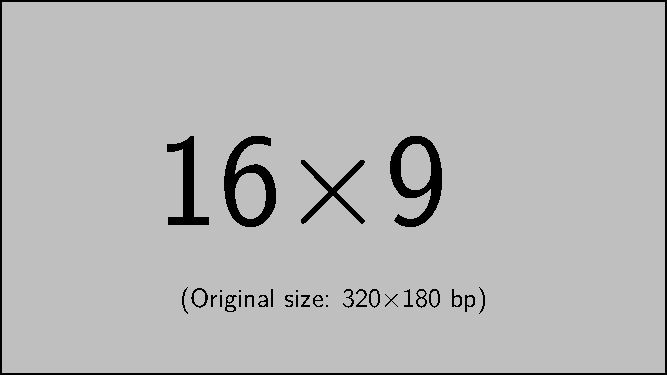
\includegraphics[width=0.88\textwidth]{figures/study-1/study-overview.pdf}
  \caption[Example full-width figure.]{Example full-width figure included from a PDF asset. Replace the file path with a legible, high-resolution PDF, PNG, or JPEG image.}
  \label{fig:study-overview}
\end{figure}

\begin{figure}[p]
  \centering
  \begin{subfigure}[t]{0.47\textwidth}
    \centering
    
\includegraphics[width=\linewidth]{figures/study-1/input.pdf}
    \caption{Input}
    \label{fig:panel-input}
  \end{subfigure}\hfill
  \begin{subfigure}[t]{0.47\textwidth}
    \centering
    
\includegraphics[width=\linewidth]{figures/study-1/reference.pdf}
    \caption{Reference}
    \label{fig:panel-reference}
  \end{subfigure}

  \vspace{5mm}

  \begin{subfigure}[t]{0.47\textwidth}
    \centering
    
\includegraphics[width=\linewidth]{figures/study-1/baseline.pdf}
    \caption{Baseline}
    \label{fig:panel-baseline}
  \end{subfigure}\hfill
  \begin{subfigure}[t]{0.47\textwidth}
    \centering
    
\includegraphics[width=\linewidth]{figures/study-1/proposed-result.pdf}
    \caption{Proposed result}
    \label{fig:panel-proposed}
  \end{subfigure}
  \caption[Example four-panel figure.]{Example four-panel figure. This caption deliberately tests \best{bold best-result text} and \runnerup{underlined runner-up text}; the plain optional caption keeps both styles out of the List of Figures.}
  \label{fig:multi-panel}
\end{figure}
\FloatBarrier

\section{Results}
\label{sec:study-one-results}

Present results in the same order as the research questions or objectives. Report
sample sizes, uncertainty, and the statistical procedure alongside point estimates.
Use tables for exact comparisons and figures for patterns; the prose should explain
the important finding rather than repeat every displayed value.

\begin{table}[htbp]
  \centering
  \caption[Example ranked result table.]{Example ranked result table with fictitious values. The caption tests \best{bold best-result text} and \runnerup{underlined runner-up text}; the plain optional caption keeps both styles out of the List of Tables. Arrows indicate the preferred direction of each metric.}
  \label{tab:result-ranking}
  \begin{threeparttable}
  \small
  \begin{tabularx}{\textwidth}{@{}l@{\hspace{4mm}}*{4}{>{\centering\arraybackslash}X}@{}}
    \toprule
    \multirow{2}{*}{\textbf{Method}} & \multicolumn{2}{c}{\textbf{Primary evaluation}} & \multicolumn{2}{c}{\textbf{External evaluation}} \\
    \cmidrule(lr){2-3}\cmidrule(l){4-5}
    & \textbf{Score $\uparrow$} & \textbf{Error $\downarrow$} & \textbf{Score $\uparrow$} & \textbf{Time (ms) $\downarrow$} \\
    \midrule
    Baseline A & 0.812 $\pm$ 0.011 & 0.184 $\pm$ 0.008 & 0.774 & 18.2 \\
    Baseline B & 0.846 $\pm$ 0.009 & \runnerup{0.151 $\pm$ 0.006} & 0.801 & \best{12.7} \\
    Baseline C & \runnerup{0.873 $\pm$ 0.007} & 0.158 $\pm$ 0.007 & \runnerup{0.829} & 16.4 \\
    Proposed method & \best{0.891 $\pm$ 0.006} & \best{0.143 $\pm$ 0.005} & \best{0.851} & \runnerup{14.1} \\
    \bottomrule
  \end{tabularx}
  \begin{tablenotes}[flushleft]\footnotesize
    \item Values are illustrative means $\pm$ standard deviations. Replace them with verified results and state the number of repetitions and statistical procedure.
  \end{tablenotes}
  \end{threeparttable}
\end{table}


Use \verb|\best{...}| and \verb|\runnerup{...}| throughout the thesis rather
than encoding rank with colour alone. This remains legible when printed in
greyscale and keeps the meaning consistent across tables.

\section{Discussion}
\label{sec:study-one-discussion}

Interpret the results in relation to the study objectives and the literature.
Use ablation studies to isolate important design choices and robustness analyses
to test sensitivity to plausible alternatives. Report negative or inconclusive
findings when they affect the interpretation.

The interpretation should connect \Cref{tab:result-ranking} to the research
questions, report uncertainty, and distinguish statistical evidence from
practical significance. Discuss study-specific limitations and keep claims within
the population, data, and conditions actually evaluated.


\chapter{Conclusions and Suggestions for Future Research}
\label{ch:conclusions}

\section{Conclusions}

The conclusion should answer the thesis objectives directly, identify the
contribution supported by each study, and explain the overall significance of the
findings. Keep the claims proportional to the evidence and avoid introducing new
experiments, citations, or arguments at this stage.

\section{Limitations}

Summarise the constraints that materially affect validity or generalisability. For
each important limitation, explain whether it may change the magnitude, direction,
or applicability of the conclusions and note any mitigation already incorporated
into the study design.

\section{Suggestions for Future Research}

Future work should follow from unresolved questions in the results and limitations.
Prioritise concrete studies that could validate, extend, or challenge the thesis
findings, and distinguish near-term follow-up experiments from broader long-term
research directions.


% PolyU's prescribed order places appendices before references.
\appendix
\chapter{Supplementary Material}
\label{app:supplementary}

Appendices are optional. This example demonstrates a table that repeats its heading across several pages. Remove this file and its \verb|\input| line from \texttt{main.tex} when no appendix is required.

\section{Multi-page Record}

\begin{longtable}{@{}>{\centering\arraybackslash}p{0.08\textwidth}p{0.24\textwidth}p{0.59\textwidth}@{}}
  \caption[Example multi-page supplementary table.]{Example multi-page supplementary table containing distinct reproducibility records and a repeated header.}
  \label{tab:appendix-long}\\
  \toprule
  \textbf{ID} & \textbf{Record} & \textbf{Information to report} \\
  \midrule
  \endfirsthead
  \multicolumn{3}{l}{\small\itshape \tablename\ \thetable\ continued from the previous page}\\
  \toprule
  \textbf{ID} & \textbf{Record} & \textbf{Information to report} \\
  \midrule
  \endhead
  \midrule
  \multicolumn{3}{r}{\small\itshape Continued on the next page}\\
  \endfoot
  \bottomrule
  \endlastfoot
  01 & Data provenance & Identify the source, collection period, licence, version, and any access restrictions for every dataset used in the thesis. \\
  02 & Cohort definition & Record inclusion and exclusion criteria, recruitment flow, and the final number of observations available for each analysis. \\
  03 & Split protocol & State how training, validation, and test partitions were formed and how leakage between related observations was prevented. \\
  04 & Preprocessing & List transformations in execution order, including normalisation constants, resizing rules, filtering, and handling of invalid records. \\
  05 & Hyperparameters & Report the search space, selection criterion, final settings, and whether tuning used information from the held-out test set. \\
  06 & Randomness & Provide random seeds and identify operations whose output may remain non-deterministic across hardware or software versions. \\
  07 & Ablation study & Define the component removed or altered, the controlled baseline, and the metric used to attribute a change in performance. \\
  08 & External validation & Describe domain differences between development and external data and state whether any adaptation occurred before evaluation. \\
  09 & Missing data & Give the amount and pattern of missingness, the chosen treatment, and a sensitivity analysis when assumptions may affect conclusions. \\
  10 & Calibration & Specify the calibration measure, binning or fitting procedure, confidence intervals, and any post-hoc adjustment applied to predictions. \\
  11 & Resource use & Report timing boundaries, repetitions, hardware, batch size, numerical precision, and peak host and accelerator memory. \\
  12 & Software environment & Preserve operating-system, compiler, library, and driver versions together with a machine-readable environment specification. \\
  13 & Ethics and consent & Record approving bodies, reference numbers, consent or waiver arrangements, and safeguards for privacy-sensitive material. \\
  14 & Artifact archive & Provide persistent locations, checksums, licences, and access instructions for code, configurations, trained models, and derived data. \\
\end{longtable}


\section{Supplementary Derivation}

Use an appendix for supporting material that is necessary for verification but
would interrupt the main argument, such as extended derivations, additional
experiments, questionnaires, or implementation details. Give every appendix item a
clear purpose and refer to it from the main text when it supports a claim.

\begin{equation}
  \widehat{\theta}=\underset{\theta\in\Theta}{\arg\min}\;\sum_{i=1}^{N}\ell\bigl(f_{\theta}(x_i),y_i\bigr).
\end{equation}


\clearpage
\printbibliography[heading=bibintoc,title={References}]

\end{document}
